\begin{center}
\LARGE\textbf{PI Summary: Jaehoon Yu}
\end{center}

%%%%%%%%%%%%%%%%%%%%%%%%%%%%%%%%%%%%%%%%%%%%%%%%5
\section*{\textbf{Accomplishments}}
%%%%%%%%%%%%%%%%%%%%%%%%%%%%%%%%%%%%%%%%%%%%%%%%%
Since I have been in transition in the past three years, my accomplishments in the Energy Frontier (EF) are also summarized here along with those in I.F. 

\noindent\textbf{Accomplishments in Energy Frontier Program}
\begin{itemize}[noitemsep,nolistsep]
\item{Graduated a Ph.D. student, Dr. Heeyeun Kim in 2015}
\item{Expect to graduate another Ph.D. student, Mr. Feremenga by the end of the current funding cycle}
\item{Served on various Higgs editorial boards as a member}
\item{Contributed to publication of a couple of $H\rightarrow WW$ papers as an author}
\item{Contributed to publication of a couple $H^{+}\rightarrow \tau+\nu$ papers as an author}
\item{Contributed to publication of exclusive production of Higgs paper as an author}
\item{Served as an ATLAS leader shifter in 2016 for 13 TeV data taking}
\item{Serving as a member of the search committee for the deputy US ATLAS Physics Support Manager}
\end{itemize}

\noindent\textbf{Accomplishments in Intensity Frontier Program}
\begin{itemize}[noitemsep,nolistsep]
\item{Co-lead Detector R$\&$D Coordination group of LBNE}
\item{Contributed to the transition from LBNE to DUNE working on collaboration governance}
\item{Organized and hosted the first off-Fermilab-site DUNE collaboration meeting at UTA}
\item{Co-leading the Beyond the Standard Model physics group of DUNE}
\item{Contributed to LBNE Physics Book}
\item{Contributed to various beam systematics and optimization studies}
\item{Contributed to LBNE/DUNE hadron monitor development}
\item{Contributed to WA105 $3\times 1 \times 1~{\rm m^{3}}$ prototype construction during the sabbatical stay in Sept. 2015 - May 2016}
\item{Lead UTA group to join WA104, ICARUS experiment}
\item {Supervised numerous undergraduate students in their contribution to the LBNF beam line systematics and optimization studies}
\item {Supervised postdoctoral fellow Dr. Animesh Chatterjee for his contributions to DUNE, LArIAT, and MiniBooNE}
\end{itemize}

%%%%%%%%%%%%%%%%%%%%%%%%%%%%%%%%%%%%%%%%%%%%%%%%%
\section*{\textbf{Milestones}}
%%%%%%%%%%%%%%%%%%%%%%%%%%%%%%%%%%%%%%%%%%%%%%%%%
\noindent\textbf{DUNE BSM Physics}
\begin{itemize}[noitemsep,nolistsep]
\item{\textbf{Complete Initial DUNE BSM Physics list document}}: Late 2016
\item{\textbf{Complete Systematic Sensitivity Studies}}: Late 2017/Early 2018
\item{\textbf{Refine Sensitivity Studies}}: Mid 2018
\item{\textbf{Contribute to writing the DUNE Technical Design Report (TDR)}}: Mid 2018
\end{itemize}

\noindent\textbf{protoDUNE Experiment}
\begin{itemize}[noitemsep,nolistsep]
\item{\textbf{Complete DP Field Cage (FC) Design and establish QA/QC Plan}}: Late 2016/Early 2017
\item{\textbf{Complete FC submodule assembly, functional prototype testing and shipping}}: Mid 2017
\item{\textbf{Detector Installation, Commissioning, and Operations}}: Late 2017 - Mid 2018
\item{\textbf{Data Taking and Analysis}}: Mid 2018 - 2019
\item{\textbf{Contribute to DUNE TDR}}: Mid 2018
\end{itemize}

\noindent\textbf{SBND Experiment}
\begin{itemize}[noitemsep,nolistsep]
\item{\textbf{Join the experiment}}: Early 2017
\item{\textbf{Detector Construction and Installation}}: Early 2018 - Mid/late 2018
\item{\textbf{Commissioning and Opeartion}}: Starting Mid/late 2018 
\item{\textbf{Data Analysis}}: 2019
\end{itemize}

\noindent\textbf{ICARUS Experiment}
\begin{itemize}[noitemsep,nolistsep]
\item{\textbf{Installation and Commissioning}}: Early 2017
\item{\textbf{Data Taking and Expert Training}}: Early 2018
\item{\textbf{NuMI Off-Axis Cross-Sections \& Dark Matter Searches}}: Early 2019
\begin{itemize}[noitemsep,nolistsep]
\item{Sensitivity Study: Late 2017}
\item{Preliminary Data Analysis for Conferences: Late 2018}
\item{Publication Result: Late 2019}
\end{itemize}

\end{itemize}

%\subsubsection{Magnetic Field Map Simulation Study in LBNF Ð Brown, Yu}
%A new graduate student, Garrett Brown has joined the physics department Ph.D. program January 2016 and was assigned in implementing the G4LBNE code for magnetic field mapping and displaying the field overlaid on LBNF beamline components. His first attempt was to sample the volume of the beamline by uniformly stepping point by point in 3D Cartesian coordinates and sampling the field value at each point by checking which volume the point was residing in and measuring the volume's field value at that point, or using 0 if there was no volume at that point. The problem he encountered was transforming the world coordinate of the 3D point to the local coordinate with respect to the geometry of the placement's volume. GEANT4 does not store any hierarchical information regarding the transformations between geometry, so it is up to the user to keep track of objects' transformations. Given the complication due to relying on correctly determining if a point was inside of the volume, he ultimately used geantino moving under the influence of the electromagnetic equation of motion and record the magnetic field value which GEANT4 provides. This method provided a placement independent magnetic field map.  Figure on the left of Fig.~\ref{if-beams} shows the result of this method in the current three horn system.  A further test of the comparisons of magnetic field map is necessary in order to verify the functionality of this software.
	
%\begin{figure}[htb]
%  \centering
%  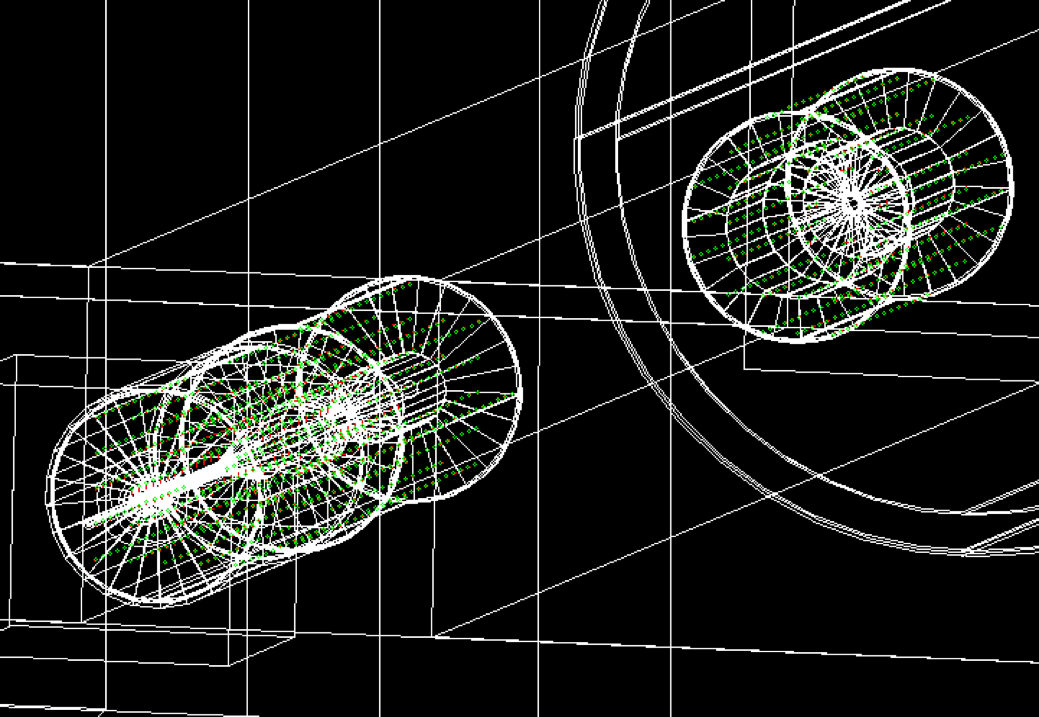
\includegraphics[width=3in]{images/if-beam1.png}
  %\includegraphics[width=3in]{imagesFigures/if-beam2.png}
% \caption{
% (left) The three polycone horns of the DUNE beamline and their magnetic fields mapped out.
% (right)}
%  \label{fig:if-beams}
%\end{figure}

%\subsubsection {Charged Pion Total Cross section on Argon in LArIAT Ð Chatterjee, Yu}
%We have studied the charged pion-nucleus total interaction cross section in liquid argon performed at the Liquid Argon In A Testbeam (LArIAT) experiment. Pion interactions with matter have been a central topic in particle physics for decades. Over the past forty years, an extensive set of pion scattering experiments have been conducted at various meson factories. LArIA[1]T program is consist of full calibration of the argon TPC in a dedicated beam line. The main goal of the LArIAT experiment is to measure pion-argon total and exclusive cross-section, 3D imaging, good particle identification and precise calorimetric reconstruction.

%The layout of the LArIAT experiment consists of two main parts: the liquid argon-related components and the beam-related components. The liquid argon-related part consists of the LArTPC detector, the liquid argon scintillation light detector, the LArTPC read-out cold electronics, the liquid argon cryostat, and the cryogenic system connected to the cryostat for liquid argon cooling and purification. The beam-related part consists of a series of beam counters such as the TOF detector, multi-wire proportional chambers (MWPCs), Cherenkov detector, and veto paddles are aligned along the LArIAT beam line for PID tagging and momentum selection. The analysis presented here of LArIAT data from Run-I aims to develop pion identification algorithms based on the information from LArIAT beamline detectors and from the pion topology in liquid argon. The procedure to achieve the measurement is based on the reconstruction and selection of charged pion events, the analysis of the calorimetric information along the track in the TPC, the vertex finding and the evaluation of the total cross section applying a "Sliced TPC" method. The result of the first measurement~\cite{if:lariat-pi-xsec} of Pion-Argon total cross-section has been shown in the plot on the left of Fig.~\ref{fig:if-animesh}.

%LArIAT has completed taking Run 2 data for 6 months from February 2016. Using the increase data set, we are studying charge sign determination of muon without using magnetic field information. The sign of the particle charge (without magnetic field) can be obtained for stopping particles in LArTPC by statistical analysis based on topological criteria. For example, $\mu^{+}$ undergo decay only, with e+ emission of known energy spectrum. Stopping $\mu^{-}$  may either decay or be captured by nuclei.

%\begin{figure}[htb]
%  \centering
  %\includegraphics[width=3in]{images/if-ch-pi-xssec-lariat.png }
  %\includegraphics[width=3in]{images/if-beam2.png}
% \caption{
% (left) First measurement of Pion-Argon Total cross-section at LArIAT
% (right) .
%  }
%  \label{fig:if-animesh}
%\end{figure}

%\subsubsection{Proton Beam Alignment Monitor Ð Chatterjee, Yu}
%Proton Beam Alignment Monitor (PBAM) will check the alignment of the proton beam in the neutrino beamline(LBNF).  We have done the simulation study of the Monitor at the beamline. Dimension of the Monitor we have consider for the simulation is $1m\times 1m$, gas gap of 1 mm thick which is filled with Ar gas. Monte-carlo simulation has been done with G4LBNE package with the v3r3p7 version. we have taken $5\times 10^{6}$~POT with the Nominal configuration, proton energy 120 GeV and horn current is 230 kA.  

%Most of the un-interacted protons are picked at the center of the Monitor, hence it will be important to design the Monitor into pixel like structure to get better position resolution of the proton at the center.  We have done the simulation of the Monitor with different pixel size to get the optimum resolution of the monitor. Optimum resolution of any pixels is considered when sigma of the position distribution is within the pixel size.  We are working with Fermilab accelerator division to finalize the monitor design. Our next step will be implementation of the monitor design.  

%\subsubsection{Software for DUNE Beyond Standard model group}
%We have developed a software framework for the study of NSI. The software is mainly based on GLOBES~\cite{if:globes} neutrino simulator.  The expected neutrino flux provided by the beam simulations group can be taken and input to the simulator for the BSM subgroups to study the physics sensitivity for each topic.  Neutrino cross-section and detector properties are taken from DUNE CDR.  We have done preliminary estimate of the constraints on the NSI parameter for DUNE. 
%%%%%%%%%%%%%%%%%%%%%%%%%%%%%%%%%%%%%%%%%%%%%%%%%
\section*{\textbf{Plans}}
%%%%%%%%%%%%%%%%%%%%%%%%%%%%%%%%%%%%%%%%%%%%%%%%%
During this funding cycle, I will be leading the DUNE program, protoDUNE DP and the ICARUS detector during the construction, installation and commissioning . In particular, I am responsible for assembly, functional testing and installation of the protoDUNE DP field cage (FC).  The submodules of the protoDUNE DP FC will be built and tested at UTA and be shipped to CERN for installation by mid 2017.  I plan on being stationed at CERN in fall 2017 together with a postdoctoral fellow and a graduate student for installation of them.  My schedule will be coordinated with P.I. Asaadi to maintain a constant level of P.I. effort on SBN and protoDUNE and to maximize the impact of our personnel resources.  Once I return to the U.S. after the stay at CERN in 2018, I will be focusing on SBN program to ensure the success of these programs and our group's role in SBND and ICARUS experiments on their construction, installation, commissioning and operation.  This plan will enable our group to maintain respectful number of personnel on both DUNE and SBN programs and enhance necessary expertise to play crucial roles in construction and eventual physics data analysis of DUNE.

The physics I will focus on in this proposal is the Low-mass Dark Matter searches in DUNE and SBN experiments, along with the cross-section analyses across the SBN jointly with P.I. Asaadi.  In particular, based on the production angle of LDM in high intensity proton beams, it is also feasible to perform a parasitic experiment in ICARUS off of the NuMI neutrino beams.   A systematic sensitivity study for DUNE LDM searches will be completed for an inclusion into the DUNE TDR.  I will lead the DUNE BSM subgroup to complete systematic and realistic sensitivity studies of various topics within the group to contribute to the DUNE TDR.


%\subsubsection{Field Cage for Proto DUNE Dual Phase LArTPC}
%We are working on the design and simulation of Field cage of Dual Phase of LArTPC for DUNE. The field cage design will be composed of field-shaping coils made with stainless steel.The coils are supported by 32 off-hanging columns of G-10CR glass fibre/epoxy-laminated sheet insulating material, built in the form of chains, and suspended from the tank deck structure, as shown in Fig.~\ref{if:dp-fc}. Each coil is designed as a series of fully welded infill tubes intended to fit between pairs of hanging support columns to form one section of the field cage. The prototype dual phase detector WA105 will be tested at 1 kV/cm over a 6-m drift.   We are simulating the field cage to provide an optimal design. We will measure electric field across the whole drift volume along with the other mechanical issues.

%\subsubsection{Data analysis with 35 ton LArTPC}
 %35-Ton LAr-TPC is a prototype detector for DUNE experiment. 35-Ton detector is placed at PC4 at Fermilab. It is mainly taking cosmic muon data with integrated TPC and photon detectors.  The detector has the success of seeing muon tracks with TPC. We are working to find the tracking efficiency of the detector. We are also working to understand the detector using the cosmic data. Complete the data analysis and include the result on 35-ton detector paper .

%\subsubsection{GosSiP and Photon Detector Coupling Studies Ð R. Musser}
%GosSiP is a simulation package for SiPMs that allows the user to vary multiple characteristic parameters of the detector. These parameters are important to understand because of their correlation to the signal that the SiPM generates. An important aspect of these parameters is their dependency on temperature, given that SiPMÕs will be working in LAr. This affects the overvoltage applied to the detector, which in turn determines the characteristic parameters. Originally, GosSiP did not have the ability to determine the effects that various temperatures have on a SiPM.  Musser was able to implement this element into the simulation based on the effect of varying temperatures on the SiPM characteristic parameters reported in Ref.~\cite{if:pd-ron, if:pd-ron2}.   The temperature dependences of each of the characterization parameters were analyzed and fit to the most appropriate functional form that reflects the dependencies. These equations were then implemented into the code that allowed GosSiP to calculate the parameters with respect to the temperature. Comparing the values of a room temperature simulation to a simulation at ${-196^{o}C}$ shows drastic variations. There was a 56\% and 7\% increase in PDE and gain respectively. Conversely, there was a 56\% and a 54\% decrease in DCR and crosstalk respectively. These changes resulted in a 69\% increase in mean charge strictly due to a decrease in temperature. With the ability to account for temperature dependence, GosSiP is now an even more valuable and accurate simulation package.

%While simulations of SiPMs are important, physical tests are needed in order to obtain a more complete picture. A total of 40 SensL SiPMs were collected for characterization tests. PCBs were designed and manufactured for testing of the SiPMs. A GUI in LabVIEW was created in order to collect and analyze the data from the SiPMs. This allows for instant analysis of the characteristic parameters, which will be verified with further analysis in ROOT. Since the boards with the SiPMs attached arrived, we have been soldering SMA connector to the boards for readout and bias voltage purposes. With a few boards completed, we have begun testing some of the SiPMs with a pulsating 420 nm LED. Figure 1 shows the output of a $6\times 6$~mm SensL SiPM to an oscilloscope that confirms the board is working correctly.

%Although the temperature dependence implementation in GosSiP is important, the SiPMs used to model the behavior are relatively old due to the rapid advancements of the SiPM technology. Complete temperature dependence studies of newer SiPMs are needed to form an even more accurate simulation package. Characterization studies of the 40 SiPMs will begin shortly. The PDE, gain, DCR, cross-talk, and after-pulse are going to be the main focus and will be calculated for every SiPM with varying bias voltage. This will ultimately lead us to study the optimized coupling for a SiPM and a scintillator.

%\subsubsection{Effect of Decay Pipe Radius to Neutrino Flux and CP Violation Sensitivity Study}

%My area of focus was the beam-line itself, located at Fermilab. Here is where the decay pipe is located, which is  a standard 2 meters in length. I began at 1 meter and increased the parameter by 0.05 meters. This data was then inputted into the graph below, which demonstrates the integrated flux as a faction of the radius. As one can observe, flux loss is noted at every increment, no matter how small the decrease from the standard 2 meters. Next I began running CP Violation Sensitivity tests on a different number of parameters. It was observed that CP Violation was higher as the radius increased to 2 meters, and no violation existed at degrees 0 and 180.

%\begin{figure}[htb]
%  \centering
  %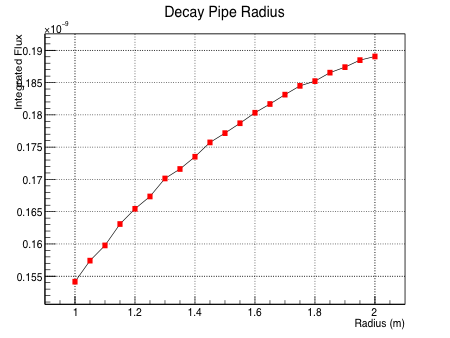
\includegraphics[width=3in]{images/decay-rad.png }
  %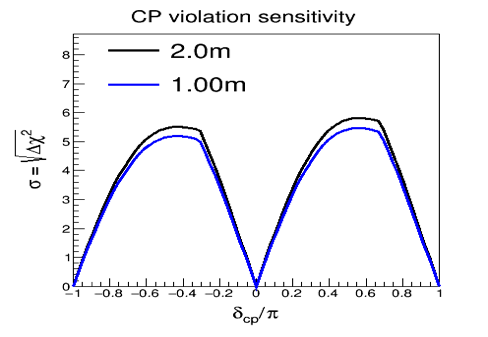
\includegraphics[width=3in]{images/cpv-sens.png}
% \caption{
% (left) The ratio of the integrated neutrino flux as a function of decay pipe radius with respect to the design radius of 2m.  
% (right) Impact to the CP violation sensitivity for change of decay pipe for 2m radius vs 1m.
%  }
%  \label{fig:if-animesh}
%\end{figure}

% references
%\bibitem{if:pd-ron}
% Ramilli, Marco. "Characterization of SiPM: Temperature Dependencies." Rapsodi. N.p., n.d. Web. 26 Aug. 2016.
%\bibitem {if:pd-ron2} Lightfoot, P. K., G. J. Barker, K. Mavrokoridis, Y. A. Ramachers, and N. J.C. Spooner. %ÓCharacterization of a Silicon Photomultiplier Device for Applications in Liquid Argon Based Neutrino Physics and %Dark Matter Searches," Arxiv. University of Sheffield, University of Warwick, n.d. Web. 26 Aug. 2016.

%\bibitem{if:lariat-exp}
%LArIAT Experiment : http://lariat.fnal.gov/;
%LarIAT: Liquid Argon In A Test Beam, http://arxiv.org/pdf/1406.5560.pdf
%\bibitem{if:lariat-pi-xsec} 
%LArIAT first Pion-Argon cross-section result: http://theory.fnal.gov/jetp/talks/Asaadi_LArIAT_WC.pdf
%\bibitem{if:globes}
%General Long Baseline Neutrino Simulator 
